\documentclass[12pt]{article}
\usepackage{amsmath,amssymb,amsthm}
\usepackage{graphicx,mathabx}
\usepackage{xcolor}
\usepackage{tikz}
\usepackage{placeins}
\usepackage{lipsum}
\usepackage[shortlabels]{enumitem}
\usepackage{placeins}
\usepackage[makeroom]{cancel}
\usepackage{mathrsfs}
\usepackage{nicefrac}
\newcommand\tab[1][1cm]{\hspace*{#1}}
\def\blankpage{%
      \clearpage%
      \thispagestyle{empty}%
      \addtocounter{page}{-1}%pdf
      \null%
      \clearpage}
\begin{document}
\title{TCSS 343 - Week 0 - Tuesday}
\author{Jake McKenzie}
\maketitle
\noindent\centerline{\textbf{Recursion and some Mathematical Review}}\\\\\\\\\\\\
\begin{center}
    ``The problem with believing is you have to believe that believing will work, you have to believe in belief". \\$\cdots$\\ Tommy Orange
\end{center}
\begin{center}
    ``So plant your own gardens and decorate your own soul, instead of waiting for someone to bring you flowers". \\$\cdots$\\ Jorge Luis Borges
\end{center}
\begin{center}
    ``It's known in theory that $\log{\log{n}}$ approaches infinity, \\but no one has ever observed it in practice". \\$\cdots$\\ Grant Sanderson (3blue1brown on youtube)
\end{center}
\begin{center}
Listen to the \textbf{MUSTN'TS}, child,\\
Listen to the \textbf{DON'TS}\\
Listen to the \textbf{SHOULDN'TS}\\
The \textbf{IMPOSSIBLES}, the \textbf{WONT'S}\\
Listen to the \textbf{NEVER HAVES}\\
Then listen close to me-\\
Anything can happen, child,\\
\textbf{ANYTHING} can be\\ 
$\dots$\\
Shel Silverstein 
\end{center}
\newpage
\begin{enumerate}
\item[0.] For the following problem I want you to trace the code. What is the final value that is printed? 
To accomplish this, \textit{\textbf{correctly}}, you will need to keep track of each the stack trace for each recursive call.
That means keeping track of the values of $x,y,u,v$ for $6$ recursive calls.
\centerline{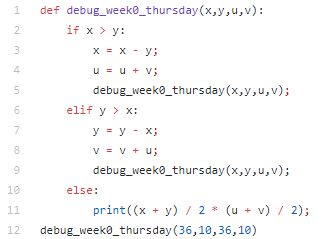
\includegraphics{debug.JPG}} 
\newpage
\item For this problem we will prove the proposition $P(n):\mathscr{F}(n) < 2^n$ where 
$\mathscr{F}(n) = \mathscr{F}(n-1) + \mathscr{F}(n-2)$ and 
$\mathscr{F}(1)=1$ and $\mathscr{F}(2) = 1$ $\forall n > 2$ 
using strong induction. 
\begin{enumerate}
\item[Step 1:] Show the ``Basis'', which means simply, show for some finite 
values that the proposition holds for those values. For instance, let $a=2$, 
show that say $P(a),P(a+1),\dots, P(5)$, that the proposition holds. These needn't 
be exhaustive but it is a good step to do to get a feel for the problem itself. 
What would be a good $a$ to pick for this problem?
\item[Step 2:] Show to inductive hypothesis, which means simply, assume $P(i)$ 
for $a \le i \le k$ where $i$ is some index variable that runs between $a$ (some 
arbitrary starting point) and $k$ (the substitution for $n$, we must replace $n$
with $k$ to for tidiness). We do this to establish our finite collection of claims 
in a tidy way. As good computer scientists we want to keep our proofs and our code 
we write as tidy as possible. This may seem like a redundant step at times but it is 
arguably the most important. What is the inductive hypothesis for this problem?
\item[Step 3: ] Show the inductive step, which means simply, prove $P(k+1)$. This 
involves introducing our inductive hypothesis into the $P(k+1)$. We assume 
that the inductive hypothesis is true. You must always introduce the inductive hypothesis into 
the inductive step. Finish the proof.
\end{enumerate}
\newpage
\item Calculate the following anti-derivatives from $1$ to $n$ with respect to $x$. 
(Because I am a nice person. Remember that $\log_2{x}=\frac{\ln{x}}{\ln{2}}$). 
I have run into all of these integrals when computing runtimes of algorithms, 
I know you didn't expect this to be so much math but please, please don't hate me. 
I added these because I care.
\begin{enumerate}
\item $6+7x+2x^2$
\item $\frac{1}{x^2}$
\item $\frac{1}{x}$
\item $2^x$ (HINT: Use the fact that $\frac{d}{dx}A^x = \ln{A}*A^x$ where $A$ is some finite real number)
\item $\log_{2}{x}$  (HINT: set $dv=1*dx$)
\end{enumerate}
\newpage
\item Emily loves figuring out all the ways to arrange dominos. Help her find all the ways to arrange dominos in that are 
$2 \times 1$ in a $2 \times 1$,$2 \times 2$,$2 \times 3$ and $2 \times 4$ grid! Avoid repeats and 
double counting by labeling each square of the domino the number of that domino. A domino can either be 
arranged vertically or horizontally in this paradigm.\\\\\\\\\\\\\\\\\\\\\\\\
\item We've had a lot of fun arranging dominos but now Emily wants a recursive formula for the ways to arrange 
$2 \times 1$ dominos. The key to finding recursive definitions is to find the answer to larger problems by finding 
the answer to smaller problems. Assume for the sake of argument that $2 \times 0$ grid has 1 way to arrange it. This 
is one of those annoying philosophical things. If I want to tile something does it exist? Is there 
zero ways or one way? We will avoid the philosophical questions and just follow the mathematics. In this case 
one is the convenient number so we will choose it arbitrarily by saying there is of course 
one way to time empty division which is $\dots$ to not do it. Is that not convincing? Well you will see, 
hopefully, that if the recurrence below holds then $D_0$ must be $1$.\\\\
$D_n = $\# of tilings of a $2 \times n =$
\newpage
\end{enumerate}
\end{document}























